\documentclass[a4paper]{article}

%% Language and font encodings
\usepackage{polski}
\usepackage[polish]{babel}
\usepackage[utf8x]{inputenc}
\usepackage[T1]{fontenc}
\usepackage{pdfpages}
\usepackage{indentfirst}
\usepackage{listings}
\usepackage{isotope}

\usepackage{csvsimple}
\setlength{\tabcolsep}{2pt}

% Adjust penalties
\brokenpenalty=1000
\clubpenalty=1000
\widowpenalty=1000

% Don't break in math expressions
\relpenalty=10000
\binoppenalty=10000

%% Sets page size and margins
\usepackage[a4paper]{geometry}

%% Useful packages
\usepackage{amsmath}
\usepackage{graphicx}
\usepackage[colorlinks=true, allcolors=blue]{hyperref}
\usepackage{booktabs}
\usepackage{cancel}
\usepackage{tikz}

\usepackage{float}

\renewcommand\thesection{\arabic{section}.}
\renewcommand\thesubsection{\arabic{section}.\arabic{subsection}.}
\renewcommand\thesubsubsection{\arabic{section}.\arabic{subsection}.\arabic{subsubsection}.}

% The following commands are not supported in PSTricks at present
% We define them conditionally, so when they are implemented,
% this pgf file will use them.
\ifx\du\undefined
  \newlength{\du}
\fi
\setlength{\du}{15\unitlength}

\newcommand{\Vsp}[1]{\vtop to #1 {}}
\newcommand{\Hsp}[1]{\hbox to #1 {}}
\newcommand{\Small}{\scriptsize}

\title{Sprawozdanie nr 8}
\date{}


\begin{document}

\begin{center}
\begin{tabular}{|p{5.5cm}|l|l|c|}
    \hline
	% Row 1.1  
	    Wydział \Vsp{4mm} &
	    \multicolumn{1}{|l}{Dzień} &
	    poniedziałek $17^{15} - 19^{30}$ &
	    Nr zespołu \\
	% Row 1.2
	    \mbox{\small{Matematyki i Nauk Informatycznych}} &
	    \multicolumn{1}{|l}{Data}  &
	    &
	    \multicolumn{1}{c|}{\Large{18}} \\
    
    \hline
	% Row 2.1 
	    Nazwisko i Imię: &
	    \Small Ocena z przygotowania &
	    \Small Ocena ze sprawozdania &
	    \Small Ocena Końcowa \\
	% Rows 2.2-2.4
	    1. Jasiński Bartosz & & &\\
	    2. Sadłocha Adrian & & & \\
	    3. Wódkiewicz Andrzej & & & \\

    \hline
    % Row 3.1
	    \multicolumn{2}{|l|}{Prowadzący \Vsp{4mm}} &
	    \multicolumn{2}{|l|}{Podpis prowadzącego} \\  
    % Row 3.2
    	\multicolumn{2}{|l|}{dr hab. Jacek Gosk} &
    	\multicolumn{2}{|l|}{} \\    	
    \hline
\end{tabular}
\label{pieczatka}
\end{center}

{\let\newpage\relax\maketitle}
\setcounter{secnumdepth}{2}


\section{Opis ćwiczenia i wstęp teoretyczny}

Celem ćwiczenia było zapoznanie się z działaniem lampy elektronowej, wykazanie zależności 
natężenia prądu anodowego diody od napięcia przyłożonego na diodę oraz wyznaczenie temperatury katody
na podstawie wykonanych pomiarów.

Przed rozpoczęciem ćwiczenia, w sali laboratoryjnej przygotowany został uprzednio układ pomiarowy,
którego schemat przedstawiono na rysunku \ref{schemat}.

\begin{figure}
\centering
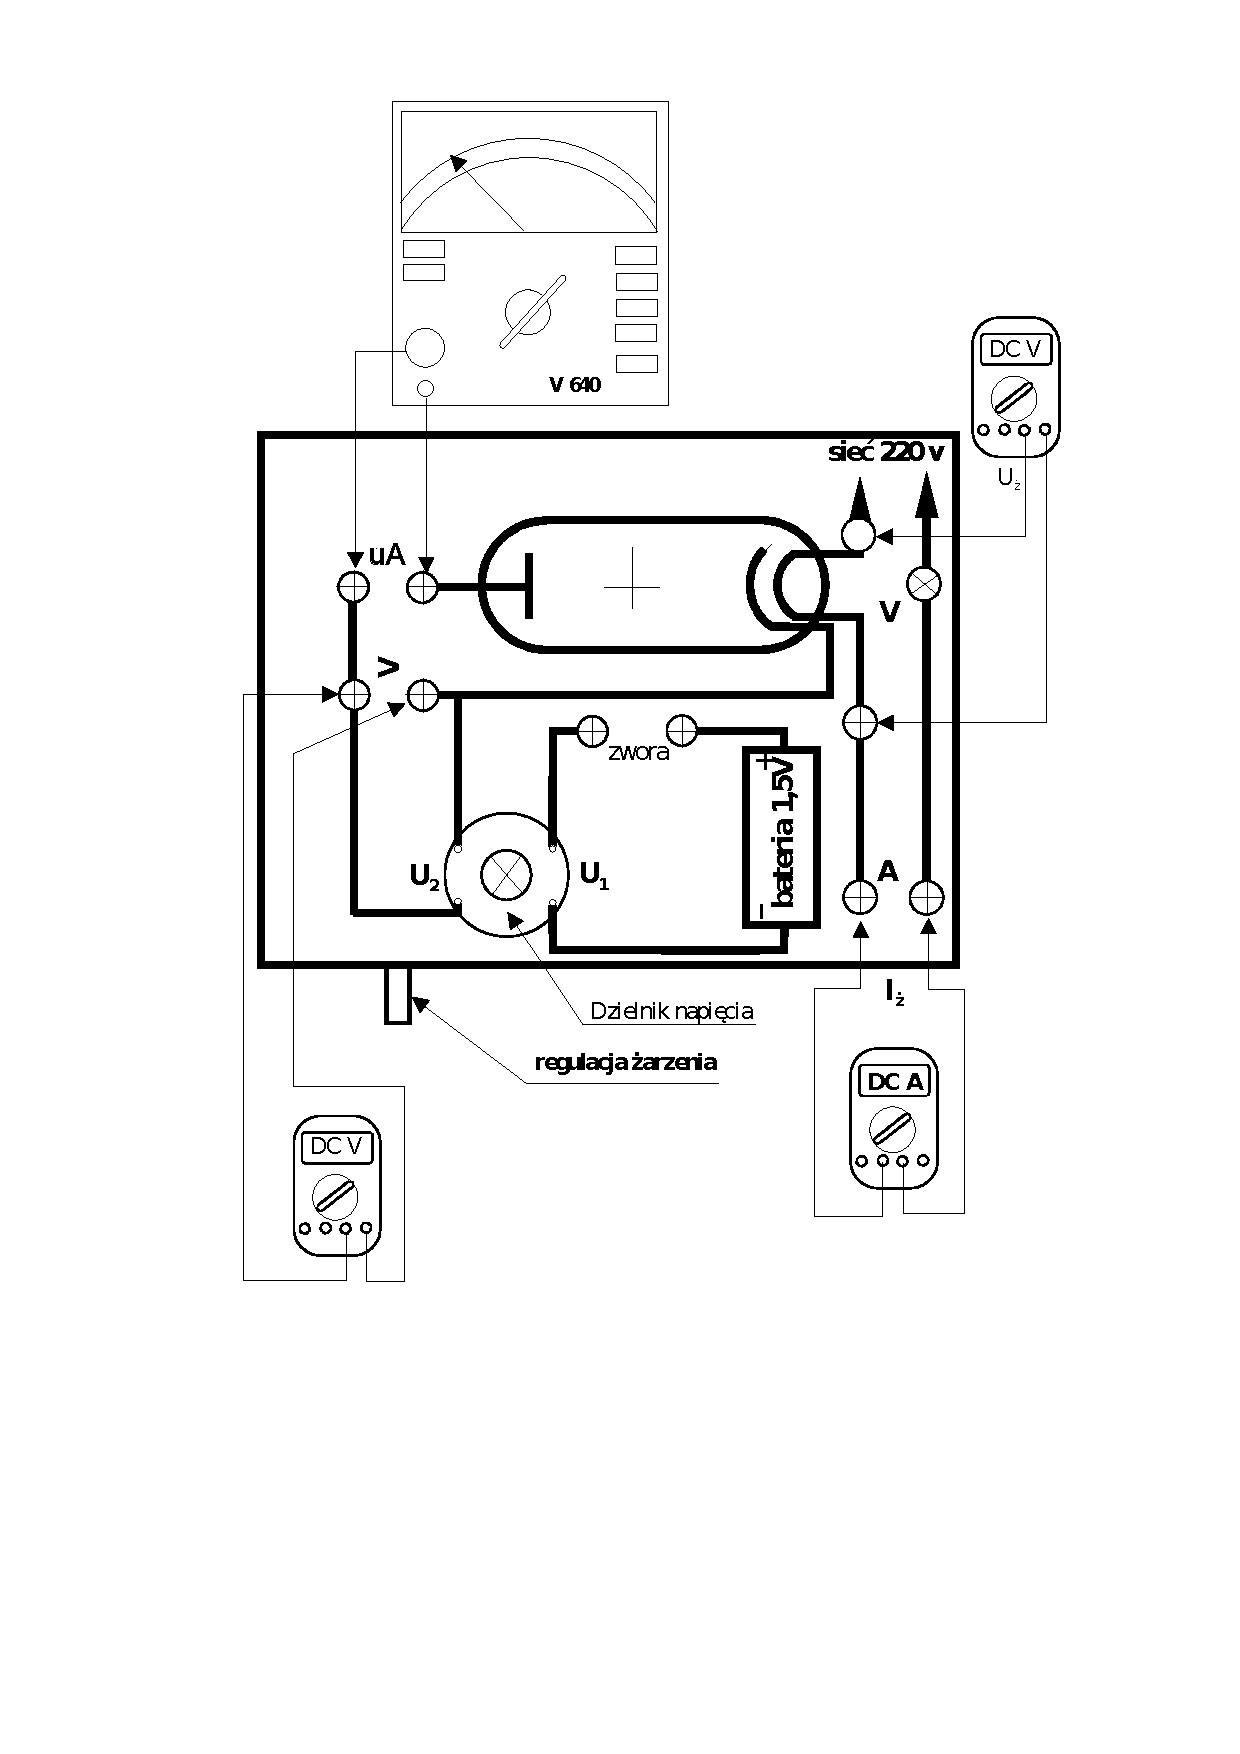
\includegraphics[scale=0.5]{schemat.png}
\caption{Schemat układu pomiarowego}
\label{schemat}
\end{figure}

Układ został przygotowany w taki sposób, aby napięcie przyłożone do lampy elektronowej hamowało
ruch elektronów opuszczających katodę (biegun dodatni baterii połączony został z katodą, a ujemny z anodą).
Budowa układu pozwalała jedynie na regulowanie wartości napięcia \textit{w jedną stronę}.
Z powodu braku możliwości zamiany polaryzacji przykładanego napięcia, nie można było wyznaczyć 
w ćwiczeniu wartości napięcia kontaktowego między okładkami.

Korzystaliśmy z przybliżenia, że elektrony wewnątrz lampy można opisać jako gaz elektronów, oraz dalej, 
z powodu znajdowania się ich w próżni nie występują oddziaływania między nimi -- jako gaz doskonały.
Były to podstawy do założenia, że prędkości elektronów przemieszczających się w kierunku anody 
mają rozkład Maxwella.

Wzór, który uwzględnia ten rozkład i posłużył w ćwiczeniu za podstawę opracowywania wyników pomiarów,
opisuje zależność między natężeniem prądu anodowego a napięciem przyłożonym do lampy.

\begin{align}
	I_a(U_a; T) = I_{a_0} \exp{\left(-\frac{e U_a}{k T}\right)}
\label{eq1}
\end{align}

gdzie $I_a$ to natężenie prądu anodowego, $U_a$ to zmienna niezależna będąca napięciem przyłożonym do lampy,
$T$ to parametr równania, będący temperaturą katody, zaś pozostałe czynniki to następujące stałe:
\begin{itemize}
\item $I_a$ -- prąd \textit{początkowy}
\item $e$ -- ładunek elementrarny z minusem
\item $k$ -- stała Boltzmanna
\end{itemize}

Analizując równanie, mozna stwierdzić, że $I_{a_0}$ to \textit{zerowe} natężenie prądu anodowego przy
braku przyłożonego dodatkowego napięcia ($U_a = 0 \text{V}$). Ponieważ napięcie $U_a$ jest hamujące,
dlatego przyjmuje w naszych rozważaniach wyłącznie wartości ujemne, stąd (pamiętając o ujemnej wartości
ładunku $e$) argument funkcji wykładniczej ma wartość ujemną. Zatem mierzona wartość $I_a$ powinna 
znajdować się w przedziale $(0; I_{a_0}]$ i maleć wraz ze zwiększaniem wartości bezwzględnej
napięcia hamującego. Dodatkowo, wraz ze zwiększaniem temperatury $T$ wykres funkcji wykładniczej
\textit{oddala} się w przedziale $(-\infty; 0)$ od osi $OX$, co wpływa na zwiększenie wartości funkcji
$I_a$ dla ustalonego $x$.

Do dalszego opracowywania wyników wyprowadzono drugi wzór ze wzoru \ref{eq1}, logarytmując równanie
stronami:

\begin{align}
	\ln{\frac{I_a}{I_{a_0}}} = -\frac{e U_a}{k T}
\label{eq2}
\end{align}

Poszukiwana była zależność liniowa, gdzie:
\begin{itemize}
\item $X = U_a$ -- zmienna niezależna
\item $Y = \ln \frac{I_a}{I_{a_0}}$ -- zmienna zależna
\item $a = -\frac{e}{kT}$ -- współczynnik kierunkowy
\end{itemize}


\section{Pomiary i wstępne obliczenia}
\section{Opracowanie wyników}
\end{document}
